\chapter{Werkzeuge}
\label{chap:Werkzeuge}
In diesem Kapitel werden die Tools vorgestellt, die in der Arbeit verwendet werden.
Dazu zählt das Anforderungsmanagement-Tool \ac{DOORS}, da es von der Siemens Mobility GmbH genutzt wird, um Anforderungen und somit auch Anwendungsregeln zu verwalten.

Das \ac{KI}-Modell, welches in dieser Arbeit erstellt und vorgestellt wird, wird in der Programmiersprache Python geschrieben.
Dieses Kapitel wird sich deshalb auch mit Python und den Bibliotheken, welche hier genutzt werden, beschäftigen und einen Überblick über diese geben.

\section{IBM Rational DOORS}
\label{chap:DOORS}

Das Anforderungsmanagement-Tool \ac{DOORS} ist ein plattformübergreifendes und unternehmensweites Tool und wird
zur Erfassung, Verknüpfung, Verfolgung, Analyse und Verwaltung von Anforderungen genutzt. \ac{DOORS} ist ein Akronym,
das für Dynamic Object-Oriented Requirements System steht. Alle Anforderungen und weitere Informationen werden in einer zentralen Datenbank
gespeichert. Innerhalb der Datenbank werden die Informationen in Modulen gespeichert. Diese Module können mithilfe von Ordnern und Projekten
organisiert werden. Ordner sind vergleichbar mit den Ordnern z.B. im Windows Explorer und können andere Ordner, Projekte oder Module
beinhalten. Ein Projekt hingegen ist ein spezieller Ordner, der alle Daten für ein entsprechendes Projekt beinhaltet. Sowohl für 
Ordner als auch für Projekte können die Zugriffsrechte individuell eingestellt werden \cite[vgl. S.173]{DOORS}. Dabei existieren die Optionen
read, modify, create, delete und administer (RMCDA). 

\subsection{Module}
Es existieren zwei verschiedene Arten von Modulen im Anforderungsmanagement-Tool \ac{DOORS}. Module, die die eigentlichen Anforderungen
beinhalten, werden Formal Module genannt. Abbildung \ref*{fig:Modul Doors} zeigt ein Beispiel für so ein Modul. Zu erkennen ist dort
ein geöffnetes Formal Module. Auf der linken Seite ist ein Explorer zu sehen, auf der rechten Seite die eigentlichen Inhalte des Moduls.
Durch den Explorer auf der linken Seite, der in einer Baumstruktur organisiert ist, wird es dem Benutzer ermöglicht leicht zu einer bestimmten
Stelle im Modul zu navigieren. Dabei können die einzelnen Sektionen auf- und zugeklappt werden \cite[vgl. S.176]{DOORS}. Die Daten auf der 
rechten Seite sind tabellarisch angeordnet. Die Spalten stellen dabei die einzelnen Attribute des Moduls dar, während die Zeilen die 
Objekte darstellen. 

Neben den Formal Modules existieren auch die Link Modules. In diesen werden Informationen über die Beziehungen zwischen einzelnen Objekten
gespeichert, was die Verfolgbarkeit von Anforderungen gewährleistet.

\begin{figure}[h]
    \centering
    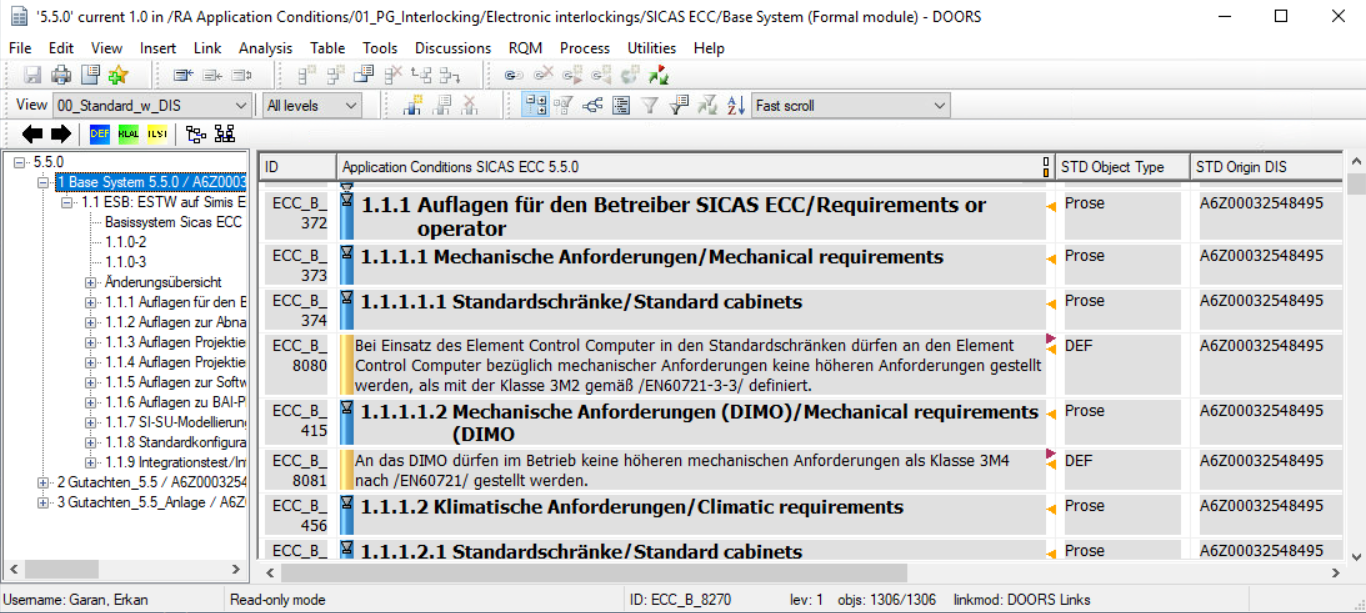
\includegraphics[width = \textwidth]{abbildungen/Modul in Doors.PNG}
    \caption{Geöffnetes Modul in \acs{DOORS}}
    \label{fig:Modul Doors}
\end{figure}

\subsection{Objekte und Attribute}
Innerhalb eines Moduls werden Daten in Objekten gespeichert. In der Regel bestehen Objekte aus mindestens zwei Spalten. Die erste 
Spalte enthält eine ID, die sich aus einem Präfix und einem Integerwert zusammensetzt. Der Integerwert wird bei jedem neu angelegtem 
Objekt inkrementiert, sodass jedem Objekt innerhalb eines Moduls eine eindeutige ID zugeordnet werden kann.
Die zweite Spalte besteht dabei entweder aus einer Sektions-Nummer und einer Überschrift, wie im ersten Objekt in der Abbildung 
\ref*{fig:Modul Doors} zu sehen ist, oder aus einem Objekt-Text, der beispielsweise eine Anforderung beinhalten kann. Ein Beispiel für 
einen Objekt-Text, der eine Anforderung beinhaltet, ist das vierte Objekt der Abbildung \ref*{fig:Modul Doors} \cite[vgl. S.178]{DOORS}.
Einem Objekt können beliebig viele weitere Attribute hinzugefügt werden. 

Attribute beinhalten relevante Informationen über Module oder Objekte. Modulattribute speichern Informationen über das Modul, wie beispielsweise
den Ersteller des Moduls, das letzte Änderungsdatum und Ähnliches. Diese Modulattribute findet der Benutzer über die Eigenschaften des Moduls, 
welche mit einem Rechtsklick auf das Modul in der grafischen Oberfläche geöffnet werden können. Objektattribute hingegen
speichern Informationen über die Objekte. In der Abbildung \ref*{fig:Modul Doors} ist die Spalte STD Object Type z.B. ein Objektattribut,
das definiert, ob es sich bei dem Objekt um eine Anforderung oder um Prosa, also z.B. eine Überschrift handelt.

\subsection{Baseline}
Eine Baseline friert den aktuellen Stand der Anforderungen eines Projekts mit ihren Attributen ein und ist eine nicht veränderbare Kopie von 
formalen Modulen \cite[vgl. S.182]{DOORS}. Baselines werden in der Regel zu Releases von Systemen oder Subsystemen erstellt \cite[vgl. S.60]{SMO-PE}. 
Wenn ein Formal Module geöffnet ist, kann der Benutzer unter File \textrightarrow{} Baseline eine Baseline erstellen oder eine bereits vorhandene 
Baseline ansehen. Abbildung \ref*{fig:Baselines} zeigt das Dialogfenster zum Öffnen bereits vorhandener Baselines. Dort wird deutlich, 
dass Baselines versioniert werden können.

\begin{figure}[H]
    \centering
    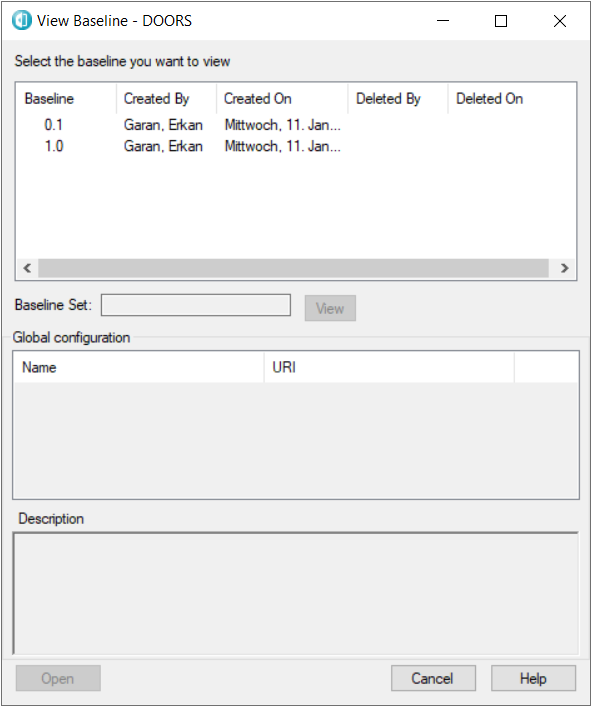
\includegraphics[scale = 0.7]{abbildungen/Baselines.PNG}
    \caption{Baselines eines Moduls in \acs{DOORS}}
    \label{fig:Baselines}
\end{figure}

\subsection{Links}
In der Abbildung \ref*{fig:Modul Doors} sind an der rechten Kante der zweiten Spalte zwei Arten von Pfeilen zu erkennen. Diese Pfeile
symbolisieren Links in \ac{DOORS}. Links sind gerichtete Verbindungen von einem Quellobjekt zu einem Zielobjekt. Sie werden in \ac{DOORS} 
genutzt, um die Verfolgbarkeit von Anforderungen zu gewährleisten. Der Benutzer kann 
dabei, ungeachtet von der Richtung des Links, vom Quellobjekt zum Zielobjekt oder andersherum navigieren \cite[vgl. S.183]{DOORS}. 
Ein nach links zeigender gelber Pfeil ist dabei ein In-Link, das heißt, dass dieses Objekt als Zielobjekt dient und ein anderes Objekt 
eine Verbindung zu diesem Objekt hat. Das Gegenstück zum In-Link ist ein Out-Link. Dieser wird in der grafischen Benutzeroberfläche von 
\ac{DOORS} als roter nach rechts zeigender Pfeil dargestellt. Hat ein Objekt einen Out-Link, heißt das, dass dieses Objekt als Quellobjekt 
dient und eine Verbindung zu einem anderen Objekt, welches als Zielobjekt dient, hat.   

\subsection{DXL}

\ac{DXL} ist eine Skript-Sprache, die ein Teil des Anforderungsmanagement-Tools \ac{DOORS} ist. Durch diese Skript-Sprache
können Skripte geschrieben werden, die als Batch-Skript ausgeführt werden können. Diese Skripte bieten neben der grafischen Benutzeroberfläche eine weitere Möglichkeit, 
um mit \ac{DOORS} zu arbeiten. Zudem besteht die Möglichkeit die grafische Benutzeroberfläche von \ac{DOORS} um neue, entwickelte Anwendungen zu
erweitern. Von der Syntax ähnelt die Sprache den Programmiersprachen C und C++ \cite[vgl. S.1]{DXL}.

\ac{DXL} wurde im Praxisprojekt zum Sammeln von Bewertungen von Anwendungsregeln aus Projekten der Siemens Mobility GmbH 
genutzt, indem Batch-Skripte geschrieben wurden. Diese Skripte haben im zentralen Projekt, das die Anwendungsregeln von Komponenten beinhaltet, die Links der Objekte
verfolgt und dort in den Modulen nach korrekt bewerteten Anwendungsregeln gesucht. Diese wurden dann nach Projekt und Komponente gruppiert und 
jeweils in neue Module geschrieben, um in Zukunft als Lösungsvorschlag für neue Projekte zu dienen. Der Inhalt dieser Module wird als Datensatz für diese Bachelorarbeit genutzt.
Ebenfalls wird \ac{DOORS} dazu benötigt, um in der grafischen Oberfläche eines Moduls mit neu importierten Anwendungsregeln ein Programm zu starten, was mit den Informationen aus dem Modul
ein weiteres Skript in der Programmiersprache Python startet. In dem Python-Skript wird das KI-Modell erstellt und angelernt. Mithilfe des Modells und mit den Daten über die Anwendungsregeln aus 
dem Modul soll das Modell dann Vorschläge zur Bewertung der Anwendungsregeln liefern.










\ac{DXL} ist eine Skript-Sprache, die ein Teil des Anforderungsmanagement-Tools \ac{DOORS} ist. Durch diese Skript-Sprache
besteht die Möglichkeit, die grafische Benutzeroberfläche von \ac{DOORS} um neue, entwickelte Anwendungen zu
erweitern. Von der Syntax ähnelt die Sprache den Programmiersprachen C und C++ \cite[vgl. S.1]{DXL}. Zudem können Skripte geschrieben werden,
die als Batch-Skript ausgeführt werden können. Diese Skripte bieten neben der grafischen Benutzeroberfläche eine weitere Möglichkeit, 
um mit \ac{DOORS} zu arbeiten. \ac{DXL} wurde im Praxisprojekt zum Sammeln von bewerteten Anwendungsregeln aus Projekten der Siemens Mobility GmbH 
genutzt, indem Batch-Skripte geschrieben wurden, welche im zentralen Projekt, das die Anwendungsregeln von Komponenten beinhaltet, die die Links der Objekte
verfolgt haben und dort in den Modulen nach korrekt bewerteten Anwendungsregeln gesucht haben. Diese wurden dann nach Projekt und Komponente gruppiert und 
jeweils in neue Module geschrieben. Der Inhalt dieser Module dient als Datensatz für diese Bachelorarbeit. Ebenfalls wird \ac{DOORS} dazu benötigt,
um in der grafischen Oberfläche eines Moduls mit neu importierten Anwendungsregeln ein Programm zu starten, was mit den Informationen aus dem Modul
ein weiteres Skript in der Programmiersprache Python startet, in der das KI-Modell erstellt und angelernt wird und mit den Daten über die Anwendungsregeln aus 
dem Modul Vorschläge zur Bewertung der Anwendungsregeln liefern soll.


\section{Python}
\label{chap:Python}

Python ist eine interpretierte, high-level, objektorientierte Programmiersprache und wird von einem Artikel 
im International Research Journal of Engineering and Technology (IRJET) als die am schnellsten wachsende Programmiersprache 
bezeichnet \cite[vgl. S.354]{Python}. Jacqueline Kazil, ehemaliges Vorstandsmitglied der Python Software Foundation,
nennt als Hauptgründe für das Wachstum der Programmiersprache die Beliebtheit von Python in den Themen \ac{ML} und Data Science \cite[vgl. S.354]{Python}.
Weitere Eigenschaften der Programmiersprache sind:
\begin{itemize}
    \item Hohe Lesbarkeit durch einfache Syntax \cite[vgl. S.354]{Python}
    \item Programme haben weniger Zeilen Code als vergleichbare Sprachen wie C \cite[vgl. S.354]{Python}
    \item hohe Flexibilität durch dynamische Typisierung \cite[vgl. S.354]{Python}
    \item Automatisches Speichermanagement \cite[vgl. S.354]{Python}
    \item läuft auf vielen verschiedenen Betriebssystemen \cite[vgl. S.355]{Python}
\end{itemize}
Die dynamische Typisierung sorgt zwar auf der einen Seite für eine erhöhte Flexibilität, da Variablen kein fester Typ bei der Deklarierung zugeordnet werden muss,
liefert aber auf der anderen Seite auch Nachteile. Durch die dynamische Typisierung kann die Ausführung eines Programms zeitintensiver werden und bei größeren 
Projekten kann es dazu kommen, dass nicht mehr genau nachvollzogen werden kann, welchen Typ eine Variable hat \cite[vgl. S.355]{Python}. Beide Nachteile sind bei der Größe
dieses Projekts aber vernachlässigbar. 

Ein großer Vorteil von Python sind die Programmierbibliotheken, die die Sprache besitzt und die importiert werden können. Für nahezu jeden Anwendungsfall existiert eine 
Bibliothek die Python um weitere Klassen und Funktionen erweitert und somit die Entwicklung von Anwendungen beschleunigt und erleichtert. Durch sie muss 
der Entwickler die Funktionalitäten, die eine Bibliothek mitbringt, nicht selber implementieren und kann stattdessen auf diese Bibliotheken zurückgreifen. 
In dieser Arbeit wurden drei Bibliotheken verwendet, die für das Erstellen von \ac{KI}-Modellen, für die Datenverarbeitung und das Visualisieren von Daten
genutzt wurden. Diese werden in den folgenden Kapiteln näher beschrieben.

Aufgrund der Beliebtheit der Sprache im Thema \ac{KI} und den Programmierbibliotheken wird Python in dieser Arbeit dazu genutzt,
die Daten aus dem Praxisprojekt zu importieren, zu verarbeiten und das \ac{KI}-Modell zu erstellen und mit den Daten anzulernen.
Eine Alternative dazu wäre die Programmiersprache R, jedoch wird hier Python bevorzugt, da Python weiter verbreitet ist und eine simplere Syntax hat und somit 
einfacher zu lesen und zu verstehen ist.

\subsection{Keras}
\label{chap:Keras}
Keras ist eine Bibliothek für die Programmiersprache Python, welche Klassen und Funktionen liefert, um verschiedene \ac{DL}-Modelle zu erstellen
und diese anschließend zu trainieren. Operationen zur Berechnung und Bearbeitung von beispielsweise Tensoren bringt diese Bibliothek nicht mit.
Stattdessen greift Keras auf andere Bibliotheken zurück, die diese Funktionalitäten mitbringen, und nutzt diese dann. Dabei ist Keras kompatibel zu mehreren
Bibliotheken dieser Art, wie zum Beispiel TensorFlow von Google oder CNTK von Microsoft. Der Entwickler kann aussuchen, welche dieser Bibliotheken
verwenden will und kann diese auch während der Entwicklung wechseln \cite[vgl. S.89ff.]{DL_PY}. François Chollet empfiehlt standardmäßig TensorFlow zu nutzen, da diese 
\glqq am weitesten verbreitet, skalierbar und ausgereift\grqq{}\cite[S.91]{DL_PY} sei. Was TensorFlow genau kann und wie es genutzt wird, ist für die Erstellung eines
\ac{DL}-Modells mit Keras nicht relevant und wird somit nicht genauer beschrieben.

Das Erstellen eines \ac{NN} mithilfe von Keras folgt dabei in der Regel den folgenden vier Schritten:
\begin{enumerate}
    \item Trainingsdatensatz definieren und in Ein- und Ausgabewerte aufteilen \cite[vgl. S.92]{DL_PY}
    \item \ac{NN} definieren, indem die einzelnen Schichten konfiguriert werden \cite[vgl. S.92]{DL_PY}
    \item Verlustfunktion, Optimierer und Metrik(Kennzahl) auswählen \cite[vgl. S.92]{DL_PY}
    \item Modell mit Trainingsdaten anlernen \cite[vgl. S.92]{DL_PY}
\end{enumerate}
Ein großer Vorteil der Bibliothek ist, dass Keras bereits die verschiedenen Schichten als Klassen mitbringt, diese also nicht vom Entwickler erst definiert werden müssen.
Der Entwickler kann dadurch einem Modell beliebig Schichten hinzufügen oder entfernen und diese nach seinen Wünschen konfigurieren. 
Die Anzahl an Neuronen innerhalb einer Schicht und die Aktivierungsfunktion der Neuronen in der Schicht werden der Schicht einfach als Parameter übergeben 
und die Aktivierungsfunktion muss ebenfalls nicht selbst definiert werden, denn da reicht es aus, den Namen der Funktion als Parameter anzugeben.
Das Auswählen der Verlustfunktion, des Optimierers und der Metrik verlaufen ebenfalls genauso einfach. Diese werden, nachdem das Modell mit seinen Schichten 
definiert wurde, ganz simpel, wie bei der Auswahl der Aktivierungsfunktion, einer Funktion als Parameter übergeben.
Genau diese Schritte werden in dieser Arbeit durchlaufen, um das \ac{KI}-System zur Bewertung von Anwendungsregeln zu erstellen und anzulernen.

\subsection{Pandas}

Um unter anderem das Importieren der Daten, welche im Praxisprojekt gesammelt wurden, zu ermöglichen, wird die Datenverarbeitungsbibliothek Pandas genutzt.
Pandas ist ein Akronym, welches für panel data steht. Diese Bibliothek basiert dabei auf Tabellen, ähnlich wie bei Excel, und bietet die Möglichkeit
Excel-Dateien, CSV-Dateien und weitere Dateitypen direkt zu importieren oder zu exportieren. Die beiden wichtigsten Datenstrukturen sind dabei die
Series und die Dataframes \cite[vgl. S.253]{NumerischesPython}. 

Series können dabei wie eine zweispaltige Tabelle verstanden werden. Die erste Spalte beinhaltet einen Index, dieser kann
dabei beliebig sein, muss also nicht wie bei einem Array aus Integer-Werten bestehen. Diese Eigenschaft unterscheidet Series von Arrays
und bietet dadurch die Möglichkeit beliebige Indizes zu nutzen und Daten somit als Key-Value-Paare zu speichern. Wird jedoch kein spezieller Index definiert,
so besteht der Index, genau wie bei einem Array, aus aufsteigenden Integer-Werten von 0 bis zur Länge der Series. In der anderen Spalte
werden die eigentlichen Werte gespeichert, diese müssen dabei alle vom selben Datentyp sein \cite[vgl. S.254f.]{NumerischesPython}. 
Weitere Eigenschaften der Datenstruktur Series sind:
\begin{itemize}
    \item Indizierung \cite[vgl. S.256]{NumerischesPython}
    \begin{itemize}
        \item über Index oder Liste von Indizes auf bestimmte Werte eines Series-Objekts zuzugreifen
    \end{itemize}
    \item Filtern nach einer Bedingung, zum Beispiel nur auf Werte zugreifen, die größer als ein Schwellwert sind \cite[vgl. S.256]{NumerischesPython}
    \item Anwendung von mathematischen Funktionen auf gesamtes Series-Objekt möglich \cite[vgl. S.256]{NumerischesPython}
\end{itemize}

Dataframes sind eine weitere Datenstruktur, die die Pandas Bibliothek mitbringt. Ein Dataframe hat, wie ein Series-Objekt, ebenfalls Ähnlichkeiten zu einer Tabelle,
dieses Mal jedoch mit einer unbegrenzten Anzahl an Spalten. Die Werte einer Spalte müssen vom selben Datentyp sein, jedoch können verschiedene Spalten 
auch verschiedene Datentypen besitzen. Da nun mehrere Spalten mit Werten vorhanden sein können, besitzen Dataframes sowohl einen Zeilen- als auch einen
Spaltenindex. Die Indizes sind wieder beliebig wählbar. Zudem können mindestens zwei Series-Objekte zu einem Dataframe
konkateniert werden \cite[vgl. S.263f.]{NumerischesPython}. Also kann über Dataframes gesagt werden, dass sie eine Datenstruktur sind, die aus mehreren einzelnen Series-Objekten bestehen.

Neben den beiden Datenstrukturen liefert die Pandas Bibliothek zahlreiche Funktionen zur Analyse, Bearbeitung und Verwaltung der gespeicherten Daten. Die in dieser Arbeit 
verwendeten Funktionen werden in Kapitel \ref*{chap:Datensatz} an den gesammelten Daten aus dem Praxisprojekt vorgestellt und erläutert.

\subsection{Matplotlib}
Zur Visualisierung von Daten wird in dieser Arbeit die Bibliothek Matplotlib für Python genutzt. Matplotlib bietet die Möglichkeit verschiedenste Diagramme und Darstellungen,
wie zum Beispiel Linien-, Balken-, Tortendiagramme und viele mehr, mit wenig Code zu erstellen. Die erstellten Diagramme können vom Entwickler zudem noch beliebig 
konfiguriert werden \cite[vgl. S.167.]{NumerischesPython}. Das Visualisieren der Daten sorgt für ein besseres Verständnis der Daten im Vergleich zu einer rein textuellen Beschreibung.

Matplotlib eignet sich vor allem in der Verwendung zusammen mit Pandas. Pandas listet Matplotlib als \glqq optionale Abhängigkeit\grqq{}, bedeutet, dass für die Verwendung
von Pandas Matplotlib nicht zwingend benötigt wird, aber es empfohlen wird \cite[vgl. S.253]{NumerischesPython}.
Beide Datenstrukturen der Pandas-Bibliothek besitzen zudem eine Plot-Funktion, also eine Funktion um ein Diagramm aus den Daten zu erstellen, 
die genutzt werden kann, wenn sowohl Pandas als auch Matplotlib als Bibliotheken importiert werden.


